\section{Overview}
\label{sec:overview}

Two key aspects influence the performance and flexibility of a multi-version
execution system: system call interception and version coordination.  We discuss
each in turn below.

\subsection{System call interception}
\label{sec:interception}

%% \begin{enumerate}[(i)]
%% \item wait for the interrupt signaling the entry to a system call;
%% \item examine the registers to determine whether the system
%% call is of interest;
%% \item for any arguments passed by reference, copy the content of
%% the memory for the process address space if necessary;
%% \item if the system call is to be skipped (or performed by the monitor
%% on behalf of the application), replace the original system call with a
%% "null" system call (\ie \stt{getpid});
%% \item restart the execution of the application to execute the system call;
%% \item wait for the interrupt signaling the exit from a system call;
%% \item obtain the process registers to read the system call return value;
%% \item for any output arguments, copy the referenced data from
%% the process address space if needed; and
%% \item continue the execution of the application.
%% \end{enumerate}

The biggest downside of existing system call monitors based on the
\ptrace interface is the performance
overhead~\cite{cox2006,orchestra09,tachyon12,mx}.  For each system
call performed by each version, the monitor has to perform several
additional system calls and interrupts in order to be notified about
system call entry and exit, copy buffers to and from the version being
monitored, nullify the system call, \etc

For CPU-intensive applications which perform very few system calls,
this overhead will be amortized, resulting in a modest
slowdown. However, for heavily I/O-bound applications,
% such as those addressing the "C10k" problem (\eg nginx or lighttpd)
the slowdown can be up to two orders of magnitude, which is
unacceptable for many real-world deployments.
%
Consequently, in order to implement a system call monitor with
acceptable overhead even for heavily I/O-bound applications, we need
to eliminate context switching to the kernel and back during
interception.  This is accomplished through a combination of binary
rewriting and an interprocess communication mechanism based on a
fast shared memory ring buffer.

%\vspace{0.1in} \noindent \textbf{Selective binary rewriting.}  
Whenever code is loaded into memory, \nx scans each code page to
selectively rewrite all system calls with jump instructions to dedicated
handlers.  Section \ref{sec:rewriting} discusses in detail the main
steps and challenges associated with this binary rewriting approach.

To further eliminate the need for additional system calls during interception,
\nx uses a shared ring buffer to communicate between versions.  This
ring buffer is heavily optimized for performance: it is stored in
memory, allows largely lock-free communication, and does not require
the dispatch of events to different queues.  These aspects are
discussed in detail in Section~\ref{sec:ipc}.



\subsection{Event-streaming architecture}
\label{sec:coordination}

\begin{figure}[t]
  \begin{center}
    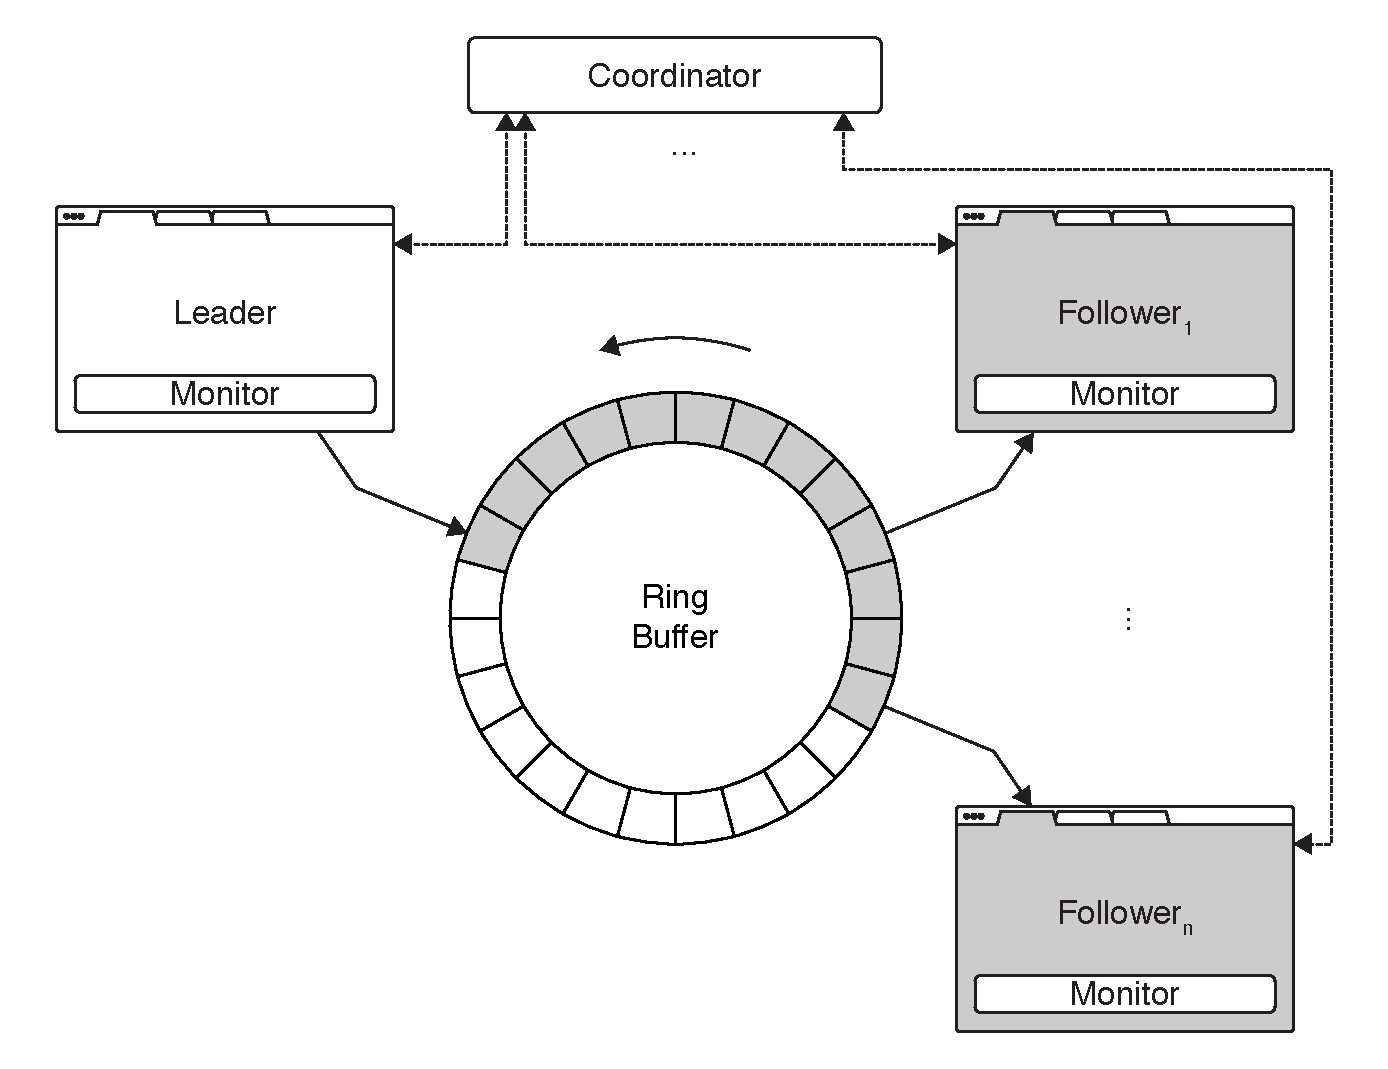
\includegraphics[width=\columnwidth]{efficient-execution/figures/architecture}
    \caption{The event-streaming architecture of \nx.}
    \label{fig:architecture}
  \end{center}
\end{figure}


In prior NVX systems, versions are typically run in lockstep, with a centralized
monitor coordinating and virtualizing their execution.  Essentially, at each
system call, the versions pass control to the monitor, which waits until all
versions reach the same system call.  Once this happens, the monitor executes
the system call and communicates the result to each individual version. The
situation when one or more versions execute a different system call or do not
execute any system call at all is seen as a divergence, which needs to be
handled by the monitor (\eg by terminating these versions or the entire
application).

There are two key disadvantages in this approach.  First, the
centralized monitor acts as a bottleneck, which can have a significant
impact on performance.  Note that in addition to the synchronization overhead,
this centralized monitor makes the multi-version application execute at the
speed of the slowest individual version.

Second, this approach is totally inflexible to any divergence in the
sequence of system calls executed across versions; this is an issue
both when running automatically-diversified variants, where certain
transformations can affect the external behavior, and when running
existing software versions, where (slight) changes in the system call
sequence can occur between versions. % (\eg extra \stt{sysconf} checks).
%% In addition, the \stt{libc} library may introduce variations between
%% the sequence of system calls, \eg by non-deterministically deciding to
%% merge two small write system calls into a single large
%% one. \todo{check if this happens non-deterministically}.

To address these limitations, \nx uses a new approach which we call
\emph{event streaming}.  In this decentralized architecture,
depicted in Figure~\ref{fig:architecture}, one of the
versions is designated as the \textit{leader}, while the others are
\textit{followers}. During execution, the leader records all system
call invocations into a shared ring buffer, which are later read by
followers to mimic the leader's external behavior
(\S\ref{sec:streaming}).

In general, any version can be the leader, although in some situations
some may be a better choice than others--\eg when running multiple
software versions in parallel, one might prefer to designate the
newest one as leader.  However, the leader can be easily replaced if
necessary, \eg if it crashes (\S\ref{sec:leader-repl}).

The only centralized component in this architecture is the
\textit{coordinator}, whose main job is to prepare the versions for
execution and establish the necessary communication channels.  At a
high level, the coordinator first loads the variants into memory,
injects several special handlers and memory objects into their address
spaces, rewrites any system calls in their code with jumps to the
special handlers and then starts executing the variants
(\S\ref{sec:setup}) in a decentralized manner.

%% recorded by one application version are shortly replayed
%% (\textit{streamed}) to the others, which keeps the log small, as
%% events which have been replayed by all versions can be discarded.
%% Similarly, the NVX context allows for the log to be kept in memory,
%% and for the replay to be done incrementally, with significant
%% performance advantages.  Event streaming is discussed in detail in
%% Section~\ref{sec:streaming}.


%% This is a variant of record-replay~\cite{scribe,jockey,geels06,r2},
%% but the NVX context allows us to overcome two of the main limitations
%% of traditional record-replay techniques, namely (1)~the
%% rapidly-growing log size, especially for system call-intensive
%% applications; and (2)~the long time necessary to replay the execution.
%% Because the multiple versions are executed concurrently, events
%% recorded by one application version are shortly replayed
%% (\textit{streamed}) to the others, which keeps the log small, as
%% events which have been replayed by all versions can be discarded.
%% Similarly, the NVX context allows for the log to be kept in memory,
%% and for the replay to be done incrementally, with significant
%% performance advantages.  Event streaming is discussed in detail in
%% Section~\ref{sec:streaming}.


\subsection{Rewrite rules for system call sequences}
\label{sec:rw}

In addition to eliminating the central monitor bottleneck, our event-streaming
architecture also supports (small) divergences between the system call
sequences of different versions.  For example, different software versions
(revisions) can be run inside an NVX environment only as long as they all issue
the same sequence of system calls~\cite{mx}.  However, software patches
sometimes change the external behavior of an application; in particular, many
divergences in system call traces fall into the following two categories:
\begin{inparaenum}[(i)]
\item \emph{addition/removal}, characterizing situations when one
  of the versions performs an additional system call (or conversely
  does not perform), typically as a consequence of an additional
  check, and
\item \emph{coalescing}, covering the situations when a (repeated)
  sequence of system calls is executed a different number of times
  in each version (\eg one version might execute two \stt{write} system calls,
  while another version executes only one \stt{write} system call to write the
  same bytes because extra buffering is used).  
\end{inparaenum}

% \begin{description}
%   \item[Addition/Removal] This class characterizes situations when one
%     of the versions performs an additional system call (or conversely
%     does not perform), typically as a consequence of an additional
%     check.
%   \item[Coalescing] This class covers the situations when a (repeated)
%     sequence of system calls is executed a different number of times
%     in each version.  E.g., one version might execute two \stt{write}
%     system calls, while another a single equivalent \stt{write} to
%     write the same bytes (\eg because extra buffering is used).  
% \end{description}

Unlike prior NVX systems that run versions in lockstep, \varan is able
to deal with such changes.  When followers process the
event sequence streamed by the leader, they can rewrite it to account
for any differences: \eg they can skip and merge system calls, or perform some
calls themselves.  We provide a flexible implementation of such rewrite rules
using Berkeley Packet Filter (BPF)~\cite{bpf} (\S\ref{sec:patternmatching}).

